In the following test experiments we evaluate the benefits of passing additional information through the layers of the hypervisor and guests for profiling. 
In the first test we show the interference on the IBM x3650 server and the Dell T410server.  
This experiment shows the degredation a guest application can experience when it at or near an I/O bound application and external I/O interference is occuring.
We examine some common counters without the proposed additional information, and the difficulties in determining that the degradation is from an external layer.

In the next two experiments, we show how we can calcuate the overhead (Equation 1) and interference (Equation 3) for an I/O bound application.  One experiment equally distributes all resources and one experiment overcommits the resources.  We expect the overcommitted system to have better performance without interference, but it should degrade much more when external layers need access to the resources.

In the final experiment we look at a case where the application is degraded due to an \emph{improper} system configuration.  Here we do not experience any external, interference.  We expect our method to not show any external interference.

\subsection{Interference - sharing resouces}
In this experiment, we show the memory and I/O interference from external systems.
From the guest domain running the benchmark, there is a significant drop in the application performance when run concurrently with external systems.  
Additionally, monitoring resources in the guest domain provides little information about the performance problems. 

First we divide the physical memory and CPUs into four equal parts and create four individual guest virtual machines (Dom1 - Dom4).  Each virtual machine is given 25\% of the availble resources so that no guest virtual machine would interfere with another machine if they were on separate physical systems.  We start only our Dom1 machine and run our experimental test with PGbench.  On our Dell server Dom1 is allocated 2GB Ram and 2 vCPU.  On the IBM server Dom1 is allocated 512MB vRAM and 1 vCPU.  

\subsubsection{DB Sizes}
Notice that when the DB size changes to an I/O bound system its performance drops significantly.  
This is due to the fact that it must fetch database rows from the disk and it is much slower.  
As the database size increases we get to a point where the application degrades into an I/O bound application.  
When experiencing interference the performance drops much more dramatically (Figure \ref{medIO}).  
\begin{figure}[h]
  \begin{center}
  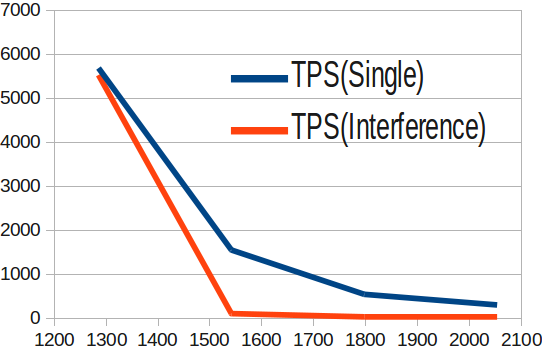
\includegraphics[width=4in]{images/MedScale.png}
  \caption{Dom1: TPS on our Dell server system with 2 vCPU and 2 GB of ram. When experiencing I/O interfernce performance drops much faster.}
  \label{medIO}
  \end{center}
\end{figure}

\begin{description}
  \item[Small DB] The working set can fit into main memory.  Performance is based on Memory.
  \item[Medium DB] The working set is swapped to disk occasionally. Performance is moving from Memory to I/O.
  \item[Large DB] Most reads need to go to disk.  Performance is based on Disk I/O.
\end{description}

\subsubsection {Show Interference}
Then we simulate external machine interference by running Dom1 concurrently with Dom2, Dom3, and Dom4. Each of the Dom2 - Dom4 systems are also configured with 2GB of RAM and 2 vCPUs.  We create a 2GB database on each external guest and run PG bench continuously to generate I/O interference.  

 We again measure the results of the benchmark on Dom1 at 3 different database sizes, while the other 3 guest domains are causing interference.  When the system is not I/O bound, there is about a 28\% drop in performance (4434 TPS - 3208 TPS) on the IBM server and little change in the Dell server (Figure \ref{fig:tps1}).  On both servers Dom1 drops to an I/O bound system faster, when there is external interference (90\% performance drop in both cases).  There is significant interference when it fully I/O bound in Dom1.

\begin{table}[h]
\begin{subtable}[h]{0.45\textwidth}
  \begin{tabular}{ l | r | r | r }
    DB Size & Single & Interfernce & Drop \\
    \hline
    Small & 4434 & 3208 & 28\% \\ \hline
    Medium & 2149 & 216 & 90\% \\ \hline
    Large & 260 & 197 & 24\% \\  \hline
    \hline
  \end{tabular}
\caption{IBM x3650 with 2GB RAM:  Each Guest domain has 512MB Allocated.}
\label{fig:tps1}
\end{subtable}
\hfill
\begin{subtable}[h]{0.45\textwidth}
  \begin{tabular}{ l | r | r | r }
    DB Size & Single & Interference & Drop \\
    \hline
    Small & 5772 & 5734 & 0.7\% \\ \hline
    Medium & 1608 & 162 & 90\% \\ \hline
    Large & 359 & 82 & 77\% \\  \hline
    \hline
  \end{tabular}
\caption{Dell T410 with 8GB RAM:  Each Guest domain has 2GB Allocated. }
\label{fig:tps2}
\end{subtable}
\caption{Dom1 TPS (Transactions Per Second) for 3 database sizes, when run as a single VM and with 3 external guests running concurrently.}
\end{table}

\subsubsection{Existing tools analysis}
\indent Trying to analyze the performance drop in Dom1 without knowing about this external interference is difficult.  
There were no changes to Dom1 when run by itself and run with other guests.  
By using the system \emph{sar} utility we can examine available memory, SwapIn and BytesIn/s to see if we can determine why the application benchmark is degraded without collecting external information (Figure \ref{fig:vmstat}).  
Memory is not used as efficiently, the system almost completely elimiates swapping data in, and also can't read as quickly from disk.  
However, there is no indication that the problem was due to an external guest and hypervisor using those resources.
A DBA looking at these numbers may conclude that kernel swap or DB tuning may fix the problem.  
The root cause of the performance drop is due to external interference, which is not known from examining the data available.
\begin{table}[h]
  \begin{tabular}{ l | r | r | r }
    VMstat & Single & Multiple & Drop \\ \hline
	Memory & 211Kb & 138Kb & 35\% \\
	SwapIn/s & 1,480 & 85 & 94\% \\
	BytesIn/s & 6,877 & 4,438 & 35\% \\
  \end{tabular}
\caption{Some resource statistics collected with vmstat on Dom1 on a Large database while running alone and with multiple systems.} 
\label{fig:vmstat}
\end{table}

% Section 7.2
\subsection{Equally sharing resources}
In the previous experiment we showed the interference that can occur when exteranl I/O interference is applied to a guest domain.
In this experiment, we repeat the previous previous experiment and pass kernel resource counter data between the hypervisor and domains.  
The results are from our IBM where each guest is configured to use 512MB of vRAM.
We run this against a 1 GB database \textbf{Large DB} in Dom1 and measure the I/O interference using the method in Section 5.  

\subsubsection{Overhead}
Calculate the overhead for the 6 counters.

\subsubsection{Interference}
Calculate the interference for the 6 counters.  Note the \emph{ms\_rd} counter which shows the interference from reading from physical disk.


% Section 7.3
\subsection{Overcommitting Resources}
In this section we test our method while resources are overcommited.  As previously mentioned, overcommitting is a common practice in hosting centers.  This allows guests that need more resources for short periods of time to have access tothose resources.  The problem is that this may cause severe degredation if multiple guests all need these resources concurrently.  

\indent For this experiment we use our Dell with 8GB of physical RAM.  
We configure all 4 domains from 2GB to 3GB of vRAM for a \emph{1.5x} overcommittment ratio.  We create a 3 GB database in each domain so that again the DB will need to read from disk often.  For this size of database expect to see a significant change in the application when the external guest domains begin 

\subsubsection{Overhead}
Calculate the overhead for the 6 counters.

\subsubsection{Interference}
Calculate the interference for the 6 counters.  Note the \emph{ms\_rd} counter which shows the interference from reading from physical disk.


% Section 7.4
\subsection{Verification without interference}
In the previous two experiments, we showed how our method can give a guest domain vital information when it is degraded from external interference.  However, what if the guest domain was degraded due to an application bug, DB change, or misconfiguration?   In that case we want our method to show that there is not any external interference.

\indent As shown previously, we use the fact that an application will degrade significantly from a memory bound system to an I/O bound system.  This is a real problem as DB can grow and needs to be purged or partitioned.  From our previous experiment with the Dell and Dom1 using 3GB vRAM.  We can use the overhead previously calculated and run 2 different tests.  The first test will use a 2GB database which will be bound by memory and will have a high TPS. The second test will have a 3GB database and will have have a much lower TPS.  Dom2 - Dom4 will be running but will not have any load or benchmark running (basically idle).










\begin{comment}
\begin{table}[h]
\begin{tabular}{ l l p{5cm} }
  Statistics & Description \\
  \hline
  /proc/diskstat & I/O statistics of block devices \\
  /proc/vmstat & Detailed virtual memory statistics\\
  \hline
\end{tabular}
\caption{Disk I/O performance counters on Linux.}
\label{tab:iocounters}
\end{table}

\subsection{}
Here we repeat the previous experiment with a large database, which is larger than available memory. We use the framework described in section 5.5 to collect I/O and virtual memory data from the /proc/diskstat and /proc/vmstat kernel statistics from all domains and the hypervisor.  From this data we can determine the impact of external I/O interference on our guest domain.\\
Before running the experiment, we need to calculate the I/O overhead by running the "dd" utility in a guest domain and collecting data without any interference.  After 3 runs we can see that the 


In this experiment we are a small virtual system: an IBM x3650 single socket quad core Intel Xeon CPU.   This machine runs CentOS 6.4 with a Xen configured kernel at 3.4.54 for Domain 0, and the Xen 4.2 hypervisor complied and packaged as part of the CentOS add on packages.   In this case Only the Dom0 is used and 3 separate memory configurations are used to show the difference between a system configured with 512MB, 1024MB, and 2048MB of ram.

\subsection{External Guest Interference}
In this experiment there we show the interference caused by running multiple virtual machines at the same time.  The following experiments are run with 4 CPUs and 2GB ruam divided between 4 virtual machines.  Each machine has 512MB and a single CPU.   In the Independent test all 4 tests are run at different times, while the concurrent test all 4 machines are run at the same time.  The reslts of the Physical machine are shown to show the Possible Maximum. 
Figure for the 512MB TPS is reported as the SUM of 4 machines.

\subsection{Guest Application Problem}
To similate a problem with a guest application we use use a misconfigured postgres database by changing the default blocksize to misalign with the guest OS ( and physical) page size.  
\textbf{--with-blocksize=BLOCKSIZE}
Set the block size, in kilobytes. This is the unit of storage and I/O within tables. The default, 8 kilobytes, is suitable for most situations; but other values may be useful in special cases. The value must be a power of 2 between 1 and 32 (kilobytes). Note that changing this value requires an initdb.  This will cause excessive reads and writes [40].  By default, the PG Block size is 8K and most (Linux) OS are configured to use 4k or 8k pages.   We use PGbench to generate an IO based workload which shows a performance degradation.  When the analyzer is run it will show a problem with the Guest Application.

\subsection{Cache Contention Problem}
Running multiple IO and memory intensive guests on the same core can result in LLC cache contention causing a performance degredation below the SLA.  PGbench can be run in a “select only” mode, in which most of the DB relations will be cached in memory.  If another DB guest is run on the same CPU socket the memory intesive application will interfere with the DB server [10].   We schedule two guest machines to run on CPU Socket 0 (core 0 and 1).  The analyzer detects the LLC cache interference and the DB server is significantly degraded below the SLA.  When moved onto separate sockets (socket 0 and 1) both the DB server and “Select Only” DB server run within the SLA.
4.6  I/O Contention 
In many cases multiple database servers could be shared on a system with multiple guests if each database only reaches peak throughput seldomly.  In this experiment we run 1 DB server per core and run the PGbench benchmark on each guest simultaneously.  If a single DB server can perform at x TPS, then it may be expected that 4 DB servers can operate at peak capacity at x/4 TPS.   Additionally, we can use PGreplay to see if we can run each system at a fraction of its speed (in this case 25\%) and achieve the same throughput on 4 separate guests.  Since there is additional overhead with the virtualiztion in DOM 0, there will be some overhead associated with the IO, and this will not be achievable.   Since a DB server synchronizes and journals the writes, each guest server will need to wait for the disk writes to complete.  The analyzer will detect the IO bottleneck issue and report problems.

\subsection{I/O Contention with ‘Disk Pinning’}
In virtualiztion it is possible to “Pin” a guest OS to a single core.  This is a way to make certain that each guest OS interference is known.  This may not be ideal in all cases, since the hypervisor may be able to better schedule guest machines on various cores (or give more cores to guests that need them).    An idea of disk pinning is similar and may (partially) alleviate some overhead in the previous experiment.  In this case, each physical disk is dedicated to a particular virtual machine, instead of a volume or raid group configured by the hypervisor.   Theoritcally, repeating the above experiment could come close to x/4 TPS except for memory cache contention.  Additionally each guest could possibly replay at 25\% of the optimal throughput on a system with 4 cores.    The issue would not be with the phyical disk I/O but with the overhead of Dom0 to schedule the disk writes.

\subsection{Virtual Cluster}
In this experiment we use a cluster of more than 1 server with a shared storage SAN server.  Each node needs an HBA with fiber connected to a fiber switch.   By running multiple guests with PG bench on the cluster server simultaneously, we can simulate an I/O contention with the shared backing store.   In a virtual cluster environment the analyzer should be able to determine that one or more guests on a particular server is exceeding their expected SLA.  Disk Pinning can also be analyzed with a large distributed backing store with multiple Logical disks (LUNs) connected with HBAs and virtualized to the guest systems.
\end{comment}
